\documentclass[a4paper,10pt]{article}
%------------------------------------------Typographie-----------------------------------------%
\usepackage[T1]{fontenc}    % césure correcte des mots accentués
\usepackage[utf8]{inputenc} % pour utiliser des caractères accentués
\usepackage[cyr]{aeguill}     % pour utiliser les guillemets français (« »)
\usepackage{xspace}           % permet à babel d'utiliser la macro xspace
\usepackage[english,francais]{babel}
\usepackage{setspace}        % pour les interlignes
\usepackage{ulem}              % pour souligner
%------------------------------------------Maths-----------------------------------------------%
\usepackage{amsmath}
%-------------------------------Graphiques et options PDF---------------------------------%
\usepackage{graphicx} % pour les graphiques  
\usepackage{xcolor}    % pour les couleurs
\usepackage{fancybox}% pour les boîtes
\usepackage{placeins}
\usepackage[utf8]{inputenc}
\usepackage{hyperref}
\usepackage{tcolorbox}
\usepackage{breqn}
\usepackage{amsfonts}
\usepackage{upgreek}
\usepackage{mathtools}
\usepackage{csquotes}
\usepackage{fancyhdr} % pour les en-têtes (haut et pied de pages)
\usepackage{fncychap} % pour modifier le style de chapitres
\usepackage{chngpage} %  
\usepackage{siunitx}
\usepackage{pdflscape}
\DeclarePairedDelimiter{\ceil}{\lceil}{\rceil}
\usepackage[width=16cm,height=24.7cm,marginparwidth=2cm,left=3cm]{geometry}

%opening
\title{INFO-H-417 : Report}
\author{Baudoux Nicolas \and Devers Marine \and Meire Wouter}

\begin{document}

\maketitle

\selectlanguage{english}
\begin{abstract}

\end{abstract}

\selectlanguage{english}
\tableofcontents

\section{Introduction}
For this assignment, we were asked to implement an external-memory merge-sort algorithm and to examine its efficiency under different parameters, such as the input file size, the size of the main memory available, the number of streams, but also many others. Before the implementation itself, we have to explore different ways to read data from, and write data to secondary memory. Then, the multi-way merge and the external multi-way merge-sort are constructed and tested. The main goal of this project is to get real-world experience with the performance of external-memory algorithms. The code of this project is fully written in \textbf{C++}.

\subsection{Environment}
We ran all our tests on one machine, here is the system environment of this machine:
\begin{figure}[ht]
\begin{minipage}[b]{.5\textwidth}
\centering
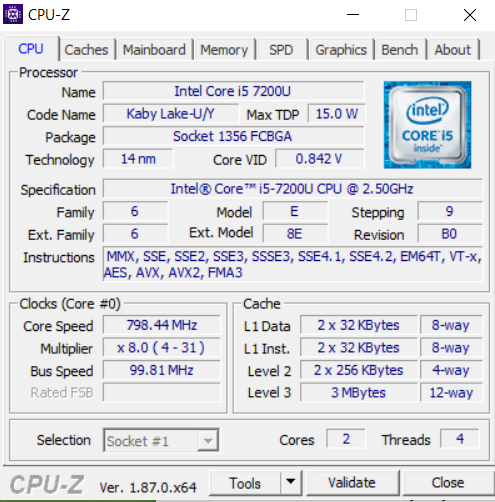
\includegraphics[width=1\textwidth]{CPU.PNG}
\caption{CPU}
\label{CPU}
\end{minipage}
\hfill
\begin{minipage}[b]{.5\textwidth}
\centering
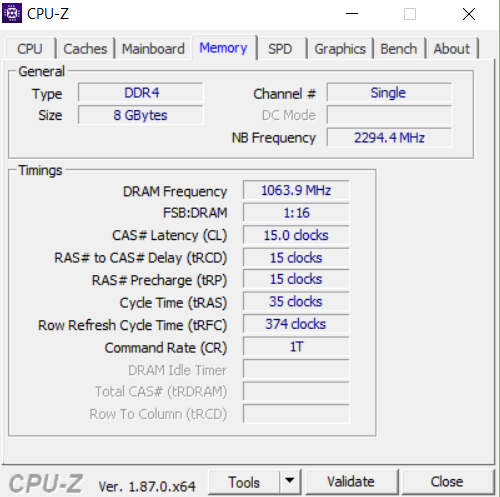
\includegraphics[width=1\textwidth]{Memory.PNG}
\caption{Memory}
\label{Memory}
\end{minipage}
\end{figure}

\subsection{Libraries used}
The following libraries are used in our project \cite{References of libraries C++}:
\begin{itemize}
\renewcommand{\labelitemi}{$\bullet$} 
\item \textbf{Boost} \cite{Boost}: this library is used to analyze every execution time of different implementations.
\item \textbf{$<$fcntl.h$>$}: this library is required to use file control options.
\item \textbf{$<$stdio$>$}: this library is required to use the \textit{fread} and \textit{fwrite} functions.
\item \textbf{$<$fstream$>$}: this library is used to operate on files. It is an input/output stream class.
\item \textbf{$<$random$>$}: this library allows us to produce random numbers using combinations of generators and distributions. 
\item \textbf{$<$bitset$>$}: a bitset stores bits. Bitsets have the feature of being able to be constructed from and converted to both integer values and binary strings.
\item \textbf{$<$windows.h$>$}: this library is required to use the function \textit{CreateFileMapping}.
\end{itemize}

\section{Observations on streams}
\subsection{Reading and writing: streams}
At first, we were asked to implement different mechanisms for reading data from, and writing data to disk. We were asked to develop \textit{streams} classes in order to read and write disk files consisting of 32-bits integers. Therefore, two types of streams are needed: the \textit{input} streams and the \textit{output} streams. The operations \textbf{open} (open an existing file for reading), \textbf{read\_next} (read the next element from the stream), and \textbf{end\_of\_stream} (a boolean operation that returns true if the end of stream has been reached) should be supported by the input stream. Also, the operations \textbf{create} (create a new file), \textbf{write} (write an element to the stream), and \textbf{close} (close the stream) should be supported by the output stream. Four distinct I/O mechanisms are used to retrieve four different implementations of the input and output streams.

\subsubsection{Read and write system calls}
For the first I/O mechanism, only one element is read or written at a time. We use the \textit{read} and \textit{write} system calls that are available through the \textit{$<$io.h$>$} header. We also use a variable called \textit{fileHandle} that is equal to $-1$ if we have not been working on a designated file.

%Stream 1: INPUT utilise le read dans biblioth�que (premier �nonc�) Si filehandle = -1 on a rien fait et si diff�rent on est en train de travailler dessus. Buffer pour lire les entiers dans le fichier (8bits par 8bits) shifter pour avoir l'entier d'origine. OUTPUT m�me chose mais en sens inverse d'abord dans buffer puis �crire dans fichier. 

\subsubsection{Read and write with its buffering mechanism}
For the second I/O mechanism, the \textit{read} and \textit{write} are performed with their own buffering mechanism. We use the \textit{fread} and \textit{fwrite} functions from the \textit{$<$stdio$>$} library. It reads integers of 32 bits and puts them into its own buffer and its writes them from the same buffer to a file using our \textit{filePointer} that points toward the open file.

%Stream 2: INPUT (deuxi�me �nonc�) utilise fread dans biblioth�que fstream on lit entier de 32bits on met dans buffer OUTPUT prend les �l�ments et les mets dans fichier via le filepointer (pointeur vers fichier ouvert) 

\subsubsection{Read and write with a buffer of size B in internal memory}
For the next I/O mechanism, the read and write are performed as in the first one explained above. However, each stream has its own buffer of size \textbf{B} in internal memory now. Instead of just reading/writting one element at a time, we can read/write \textbf{B} elements at a time. When the buffer empties itself, the following \textbf{B} elements can be read from the file. When the buffer becomes full, the following \textbf{B} elements can be written to the open file.

%Stream 3: INPUT (troisi�me �nonc�) m�me chose que deux sauf la taille du buffer voir �nonc� 

\subsubsection{Memory mapping}
The last I/O mechanism is implemented by performing \textit{read} and \textit{write} with the mapping and the unmapping of a \textbf{B} element portion of the file into internal memory through memory mapping.

%Stream 4: INPUT utilise windows.h voir �nonc� (quatri�me) encore � faire

%Tous les fichiers sont �crits en binaire
%Pch.h librairies utilis�es, moyen diff�rents de faire input et output (sauf exceptions) On cr�e un fichier random de base qui contient des entiers sign�s g�n�r�s de mani�re al�atoire pour tester (c'est une classe). 4 moyens diff�rents de lire et �crire. Input = Lire et Output = �crire.  

%Classe Benchmarking pour calculer le temps et faire comparaisons
%Tableau comparatif

\subsection{Expected behaviour}
%N grand = foireux. B grand = bien, mieux sauf si on d�passe espace dispo dans m�moire interne. k grand = foireux Si k=10, 2x fois plus lent que k=5? On dirait plus que 2x, car pleins de trucs � faire (ex: switch avec disque dur...) Performance sera plus que doubl�e. Diff�rence si utilisation de disque SSD? Acc�s � quel espace dans m�moire vive?
\subsection{Experimental observations}

\begin{landscape}
\newpage
\numberwithin{table}{section}
\begin{table}[!h]
\centering
  \begin{tabular}{|c|c|c|c|c|c|c|c|c|}
    \hline
    & Write 1 & Read 1 & Write 2 & Read 2 & Write 3 & Read 3 & Write 4 & Read 4\\
    \hline
    Average ($\mu$s) & & & & & & & & \\
     \hline
  \end{tabular}
  \caption{Read and write of 10 values with a buffer size = 512}
\end{table}

\begin{table}[!h]
\centering
  \begin{tabular}{|c|c|c|c|c|c|c|c|c|}
    \hline
    & Write 1 & Read 1 & Write 2 & Read 2 & Write 3 & Read 3 & Write 4 & Read 4\\
    \hline
    Average ($\mu$s) & & & & & & & & \\
     \hline
  \end{tabular}
  \caption{Read and write of 10 values with a buffer size = 512}
\end{table}

\begin{table}[!h]
\centering
  \begin{tabular}{|c|c|c|c|c|c|c|c|c|}
    \hline
    & Write 1 & Read 1 & Write 2 & Read 2 & Write 3 & Read 3 & Write 4 & Read 4\\
    \hline
    Average ($\mu$s) & & & & & & & & \\
     \hline
  \end{tabular}
  \caption{Read and write of 10 values with a buffer size = 512}
\end{table}

\begin{table}[!h]
\centering
  \begin{tabular}{|c|c|c|c|c|c|c|c|c|}
    \hline
    & Write 1 & Read 1 & Write 2 & Read 2 & Write 3 & Read 3 & Write 4 & Read 4\\
    \hline
    Average ($\mu$s) & & & & & & & & \\
     \hline
  \end{tabular}
  \caption{Read and write of 10 values with a buffer size = 512}
\end{table}

\begin{table}[!h]
\centering
  \begin{tabular}{|c|c|c|c|c|c|c|c|c|}
    \hline
    & Write 1 & Read 1 & Write 2 & Read 2 & Write 3 & Read 3 & Write 4 & Read 4\\
    \hline
    Average ($\mu$s) & & & & & & & & \\
     \hline
  \end{tabular}
  \caption{Read and write of 10 values with a buffer size = 512}
\end{table}

\begin{table}[!h]
\centering
  \begin{tabular}{|c|c|c|c|c|c|c|c|c|}
    \hline
    & Write 1 & Read 1 & Write 2 & Read 2 & Write 3 & Read 3 & Write 4 & Read 4\\
    \hline
    Average ($\mu$s) & & & & & & & & \\
     \hline
  \end{tabular}
  \caption{Read and write of 10 values with a buffer size = 512}
\end{table}

\begin{table}[!h]
\centering
  \begin{tabular}{|c|c|c|c|c|c|c|c|c|}
    \hline
    & Write 1 & Read 1 & Write 2 & Read 2 & Write 3 & Read 3 & Write 4 & Read 4\\
    \hline
    Average ($\mu$s) & & & & & & & & \\
     \hline
  \end{tabular}
  \caption{Read and write of 10 values with a buffer size = 512}
\end{table}

\begin{table}[!h]
\centering
  \begin{tabular}{|c|c|c|c|c|c|c|c|c|}
    \hline
    & Write 1 & Read 1 & Write 2 & Read 2 & Write 3 & Read 3 & Write 4 & Read 4\\
    \hline
    Average ($\mu$s) & & & & & & & & \\
     \hline
  \end{tabular}
  \caption{Read and write of 10 values with a buffer size = 512}
\end{table}

\begin{table}[!h]
\centering
  \begin{tabular}{|c|c|c|c|c|c|c|c|c|}
    \hline
    & Write 1 & Read 1 & Write 2 & Read 2 & Write 3 & Read 3 & Write 4 & Read 4\\
    \hline
    Average ($\mu$s) & & & & & & & & \\
     \hline
  \end{tabular}
  \caption{Read and write of 10 values with a buffer size = 512}
\end{table}

\begin{table}[!h]
\centering
  \begin{tabular}{|c|c|c|c|c|c|c|c|c|}
    \hline
    & Write 1 & Read 1 & Write 2 & Read 2 & Write 3 & Read 3 & Write 4 & Read 4\\
    \hline
    Average ($\mu$s) & & & & & & & & \\
     \hline
  \end{tabular}
  \caption{Read and write of 10 values with a buffer size = 512}
\end{table}

\begin{table}[!h]
\centering
  \begin{tabular}{|c|c|c|c|c|c|c|c|c|}
    \hline
    & Write 1 & Read 1 & Write 2 & Read 2 & Write 3 & Read 3 & Write 4 & Read 4\\
    \hline
    Average ($\mu$s) & & & & & & & & \\
     \hline
  \end{tabular}
  \caption{Read and write of 10 values with a buffer size = 512}
\end{table}

\begin{table}[!h]
\centering
  \begin{tabular}{|c|c|c|c|c|c|c|c|c|}
    \hline
    & Write 1 & Read 1 & Write 2 & Read 2 & Write 3 & Read 3 & Write 4 & Read 4\\
    \hline
    Average ($\mu$s) & & & & & & & & \\
     \hline
  \end{tabular}
  \caption{Read and write of 10 values with a buffer size = 512}
\end{table}

\begin{table}[!h]
\centering
  \begin{tabular}{|c|c|c|c|c|c|c|c|c|}
    \hline
    & Write 1 & Read 1 & Write 2 & Read 2 & Write 3 & Read 3 & Write 4 & Read 4\\
    \hline
    Average ($\mu$s) & & & & & & & & \\
     \hline
  \end{tabular}
  \caption{Read and write of 10 values with a buffer size = 512}
\end{table}

\begin{table}[!h]
\centering
  \begin{tabular}{|c|c|c|c|c|c|c|c|c|}
    \hline
    & Write 1 & Read 1 & Write 2 & Read 2 & Write 3 & Read 3 & Write 4 & Read 4\\
    \hline
    Average ($\mu$s) & & & & & & & & \\
     \hline
  \end{tabular}
  \caption{Read and write of 10 values with a buffer size = 512}
\end{table}
\end{landscape}

\subsection{Discussion of expected behaviour vs experimental observations}

\section{Observations on multi-way merge sort}
\subsection{Expected behaviour}
\subsection{Experimental observations}
\subsection{Discussion of expected behaviour vs experimental observations}

\section{Conclusion}

\newpage
\begin{thebibliography}{3}

\bibitem{Boost}
\bsc{Rene Rivera}, \emph{Boost Library Documentation} [Internet]. 2005 [Consulted on the 27th November 2018]\\
Available on:
\url{https://www.boost.org/doc/libs/}

\bibitem{References of libraries C++}
\bsc{Cpp Reference}, \emph{A list of open source C++ libraries} [Internet]. 2018 [Consulted on the 11th December 2018]\\
Available on:
\url{https://en.cppreference.com/w/cpp/links/libs}

\bibitem{Example}
\bsc{Author's Name}, \emph{Title of the source} [where was the source found]. 2018 [Consulted on the 15th November 2018]\\
Available on:
\url{http://google.com}

\end{thebibliography}

\end{document}
